%
% homologie.tex -- Homologie eines Komplexes
%
% (c) 2021 Prof Dr Andreas Müller, Hochschule Rapperswil
%
\section{Homologie
\label{buch:section:homologie}}
\rhead{Homologie}
Die Idee der Trangulation ermöglicht, komplizierte geometrische 
Objekte mit einem einfachen ``Gerüst'' auszustatten und so zu
analysieren. 
Projiziert man ein mit einer Kugel konzentrisches Tetraeder auf die
Kugel, entsteht eine Triangulation der Kugeloberfläche.
Statt eine Kugel zu studieren, kann man also auch ein Tetraeder untersuchen.

Das Gerüst kann natürlich nicht mehr alle Eigenschaften des ursprünglichen
Objektes wiedergeben.
Im Beispiel der Kugel geht die Information darüber, dass es sich um eine
glatte Mannigfaltigkeit handelt, verloren.
Was aber bleibt, sind Eigenschaften des Zusammenhangs.
Wenn sich zwei Punkte mit Wegen verbinden lassen, dann gibt es auch eine
Triangulation mit eindimensionalen Simplices, die diese Punkte als Ecken
enthalten, die sich in der Triangulation mit einer Folge von Kanten
verbinden lassen.
Algebraisch bedeutet dies, dass die beiden Punkte der Rand eines 
Weges sind.
Fragen der Verbindbarkeit von Punkten mit Wegen lassen sich also
dadurch studieren, dass man das geometrische Objekt auf einen Graphen
reduziert.

In diesem Abschnitt soll gezeigt werden, wie diese Idee auf höhere
Dimensionen ausgedehnt werden.
Es soll möglich werden, kompliziertere Fragen des Zusammenhangs, zum
Beispiel das Vorhandensein von Löchern mit algebraischen Mitteln
zu analysieren.

%
% homologieketten.tex
%
% (c) 2021 Prof Dr Andreas Müller, OST Ostschweizer Fachhochschule
%
\subsection{Homologie eines Kettenkomplexes
\label{buch:subsection:homologie-eines-kettenkomplexes}}
Wegzusammenhang lässt sich untersuchen, indem man in der Triangulation
nach Linearkombinationen von Kanten sucht, die als Rand die beiden Punkte
haben.
Zwei Punkte sind also nicht verbindbar und liegen damit in verschiedenen
Komponenten, wenn die beiden Punkte nicht Rand irgend einer
Linearkombination von Kanten sind.
Komponenten können also identifiziert werden, indem man unter allen
Linearkombinationen von Punkten, also $C_0$ all diejenigen ignoriert,
die Rand einer Linearkombinationv on Kanten sind, also $\partial_1C_1$.
Der Quotientenraum $H_0=C_0/\partial_1C_1$ enthält also für jede Komponente
eine Dimension.

Eine Dimension höher könnten wir danach fragen, ob sich ein geschlossener
Weg zusammenziehen lässt.
In der Triangulation zeichnet sich ein geschlossener Weg dadurch aus,
dass jedes Ende einer Kante auch Anfang einer Folgekante ist, dass also
der Rand der Linearkombination von Kanten 0 ist.
Algebraisch bedeutet dies, dass wir uns für diejenigen Linearkombinationen
$z\in C_1$ interessieren, die keinen Rand haben, für die also $\partial_1z=0$
gilt.

\begin{definition}
Die Elemente von
\[
Z_k
=
Z_k^C
=
\{z\in C_k \mid \partial_k z = 0\}
=
\ker \partial_k
\]
heissen die {\em ($k$-dimensionalen) Zyklen} von $C_*$.
\end{definition}

In einem Dreieck ist der Rand ein geschlossener Weg, der sich zusammenziehen
lässt, indem man ihn durch die Dreiecksfläche deformiert.
Entfernt man aber die Dreiecksfläche, ist diese Deformation nicht mehr
möglich.
Einen zusammenziehbaren Weg kann man sich also als den Rand eines Dreiecks
einer vorstellen.
``Löcher'' sind durch geschlossene Wege erkennbar, die nicht Rand eines
Dreiecks sein können.
Wir müssen also ``Ränder'' ignorieren.

\begin{definition}
Die Elemente von
\[
B_k
=
B_k^C
=
\{\partial_{k+1}z \mid C_{k+1}\}
=
\operatorname{im} \partial_{k+1}
\]
heissen die {\em ($k$-dimensionalen) Ränder} von $C_*$.
\end{definition}

Algebraisch ausgedrückt interessieren uns also nur Zyklen, die selbst
keine Ränder sind.
Der Quotientenraum $Z_1/B_1$ ignoriert unter den Zyklen diejenigen, die
Ränder sind, drückt also algebraisch die Idee des eindimensionalen
Zusammenhangs aus.
Wir definieren daher

\begin{definition}
Die $k$-dimensionale Homologiegruppe des Kettenkomplexes $C_*$ ist
\[
H_k(C) = Z_k/B_k = \ker \partial_k / \operatorname{im} \partial_{k+1}.
\]
Wenn nur von einem Kettenkomplex die Rede ist, kann auch $H_k(C)=H_k$
abgekürzt werden.
\end{definition}

% XXX Visualisierung Zyklen/Ränder, Klassen von Zyklen, die sich um einen
% XXX Rand unterscheiden

Die folgenden zwei ausführlichen Beispiele sollen zeigen, wie die
Homologiegruppe $H_2$ die Anwesenheit eines Hohlraumes detektieren kann,
der entsteht, wenn man aus einem Tetraeder das innere entfernt.

\begin{beispiel}
\begin{figure}
\centering
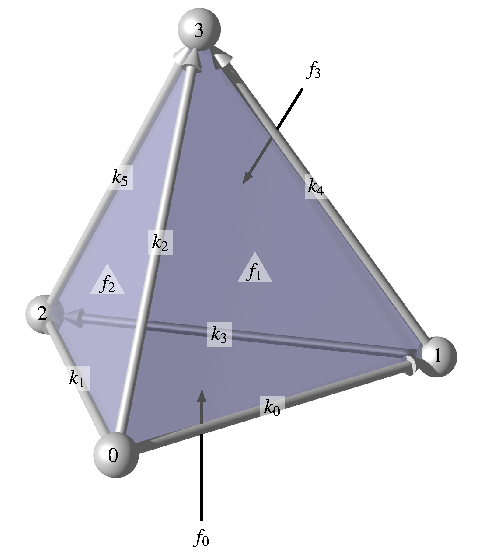
\includegraphics{chapters/95-homologie/images/tetraeder.pdf}
\caption{Triangulation eines Tetraeders, die Orientierung von Kanten
und Seitenflächen ist immer so gewählt, dass die Nummern der Ecken
aufsteigend sind.
\label{buch:homologie:tetraeder:fig}}
\end{figure}
Ein Tetraeder ist ein zweidmensionales Simplex, wir untersuchen seinen
Kettenkomplex und bestimmen die zugehörigen Homologiegruppen.
Zunächst müssen wir die einzelnen Mengen $C_k$ beschreiben und verwenden
dazu die Bezeichnungen gemäss Abbildung~\ref{buch:homologie:tetraeder:fig}.
$C_0$ ist der vierdimensionale Raum aufgespannt von den vier Ecken 
$0$, $1$, $2$ und $3$ des Tetraeders.
$C_1$ ist der sechsdimensionale Vektorraum der Kanten 
\[
k_0 = [0,1],\quad
k_1 = [0,2],\quad
k_2 = [0,3],\quad
k_3 = [1,2],\quad
k_4 = [1,3],\quad
k_5 = [2,3]
\]
Der Randoperator $\partial_1$ hat die Matrix
\[
\partial_1
=
\begin{pmatrix*}[r]
-1&-1&-1& 0& 0& 0\\
 1& 0& 0&-1&-1& 0\\
 0& 1& 0& 1& 0&-1\\
 0& 0& 1& 0& 1& 1
\end{pmatrix*}.
\]

Wir erwarten natürlich, dass sich zwei beliebige Ecken verbinden lassen,
dass es also nur eine Komponente gibt und dass damit $H_1=\Bbbk$ ist.
Dazu beachten wir, dass das Bild von $\partial_1$ genau aus den Vektoren
besteht, deren Komponentensumme $0$ ist.
Das Bild $B_0$ von $\partial_1$ ist daher die Lösungsmenge der einen
Gleichung
\(
x_0+x_1+x_2+x_3=0.
\)
Der Quotientenraum $H_0=Z_0/B_0 = C_0/\operatorname{im}\partial_1$
ist daher wie erwartet eindimensional.

Wir bestimmen jetzt die Homologiegruppe $H_1$.
Da sich im Tetraeder jeder geschlossene Weg zusammenziehen lässt,
erwarten wir $H_1=0$.

Die Menge der Zyklen $Z_1$ wird bestimmt, indem man die Lösungsmenge
des Gleichungssystems $\partial_1z=0$ bestimmt.
Der Gauss-Algorithmus für die Matrix $\partial_1$ liefert das
Schlusstableau
\[
\begin{tabular}{|>{$}c<{$}>{$}c<{$}>{$}c<{$}>{$}c<{$}>{$}c<{$}>{$}c<{$}|}
\hline
k_0&k_1&k_2&k_3&k_4&k_5\\
\hline
   1&  0&  0& -1& -1& \phantom{-}0\\
   0&  1&  0&  \phantom{-}1&  \phantom{-}0& -1\\
   0&  0&  1&  \phantom{-}0&  \phantom{-}1&  \phantom{-}1\\
   0&  0&  0&  \phantom{-}0&  \phantom{-}0&  \phantom{-}0\\
\hline
\end{tabular}
\]
Daraus lassen sich drei linear unabhängig eindimensionale Zyklen ablesen,
die zu den Lösungsvektoren
\[
z_1
=
\begin{pmatrix*}[r]
1\\
-1\\
0\\
1\\
0\\
0
\end{pmatrix*},
\qquad
z_2
=
\begin{pmatrix*}[r]
1\\
0\\
-1\\
0\\
1\\
0
\end{pmatrix*},
\qquad
z_3
=
\begin{pmatrix*}[r]
0\\
1\\
-1\\
0\\
0\\
1
\end{pmatrix*}
\]
gehören.

$C_2$ hat die vier Seitenflächen
\[
f_0=[0,1,2],\quad
f_1=[0,1,3],\quad
f_2=[0,2,3],\quad
f_3=[1,2,3]
\]
als Basis.
Der zweidimensionale Randoperator ist die $6\times 4$-Matrix 
\[
\partial_2
=
\begin{pmatrix*}[r]
 1& 1& 0& 0\\
-1& 0& 1& 0\\
 0&-1&-1& 0\\
 1& 0& 0& 1\\
 0& 1& 0&-1\\
 0& 0& 1& 1
\end{pmatrix*}.
\]
Man kann leicht nachrechnen, dass $\partial_1\partial_2=0$ ist, wie es
für einen Kettenkomplex sein muss.

Um nachzurechnen, dass die Homologiegruppe $H_1=0$ ist, müssen wir jetzt 
nachprüfen, ob jeder Zyklus in $Z_1$ auch Bild der Randabbildung $\partial_2$
ist.
Die ersten drei Spalten von $\partial_2$ sind genau die drei Zyklen
$z_1$, $z_2$ und $z_3$.
Insbesondere lassen sich alle Zyklen als Ränder darstellen, die
Homologiegruppe $H_1=0$ verschwindet.

Die Zyklen in $C_2$ sind die Lösungen von $\partial_2z=0$.
Der Gauss-Algorithmus für $\partial_2$ liefert das -Tableau
\[
\begin{tabular}{|>{$}c<{$}>{$}c<{$}>{$}c<{$}>{$}c<{$}|}
\hline
f_0&f_1&f_2&f_3\\
\hline
1&0&0& \phantom{-}1\\
0&1&0&-1\\
0&0&1& \phantom{-}1\\
0&0&0& \phantom{-}0\\
0&0&0& \phantom{-}0\\
0&0&0& \phantom{-}0\\
\hline
\end{tabular}
\]
Daraus liest man ab, dass es genau einen Zyklus nämlich
\[
z
=
\begin{pmatrix*}[r]
-1\\1\\-1\\1
\end{pmatrix*}
\]
$Z_2$ besteht also aus Vielfachen des Vektors $z$.

Da es nur ein zweidimensionales Simplex gibt, ist $C_3$ eindimensional.
Die Randabbildung $\partial_3$ hat die Matrix
\[
\partial_3
=
\begin{pmatrix*}[r]
1\\
-1\\
1\\
-1
\end{pmatrix*}.
\]
Die Zyklen $Z_2$ und die Ränder $B_2$ bilden also dieselbe Menge, auch
die Homologie-Gruppe $H_2$ ist $0$.

Da es keine vierdimensionalen Simplizes gibt, ist $B_3=0$.
Die Zyklen $Z_3$ bestehen aus den Lösungen von $\partial_3w=0$, da
aber $\partial_3$ injektiv ist, ist $Z_3=0$.
Daher ist auch $H_3=0$.
\end{beispiel}

\begin{beispiel}
Für dieses Beispiel entfernen wir das Innere des Tetraeders, es entsteht
ein Hohlraum.
Am Kettenkomplex der Triangulation ändert sich nur, dass $C_3$ jetzt 
nur noch den $0$-Vektor enthält.
Das Bild $B_2=\operatorname{im}\partial_3$ wird damit auch $0$-dimensional,
während es im vorigen Beispiel eindimensional war.
Die einzige Änderung ist also in der Homologiegruppe 
$H_2 = Z_2/B_2 = Z_2 / \{0\} \simeq \Bbbk$.
Die Homologiegruppe $H_2$ hat jetzt Dimension $1$ und zeigt damit den
Hohlraum an.
\end{beispiel}

\subsection{Basiswahl
\label{buch:subsection:basiswahl}}
Die Definition der Homologiegruppen $H_k(C)$ als Quotient von
Vektorräumen ist ziemlich abstrakt.
Sie besteht aus Klassen von Zyklen, die sich höchstens um einen
Rand unterscheiden.
Indem wir eine geeignete Basis wählen, können wir konkrete Zyklen
identifizieren, die eine Basis für den Vektorraum $H_k(C)$ bilden.
Dies soll im Folgenden schrittweise durchgeführt werden.

\begin{figure}
\centering
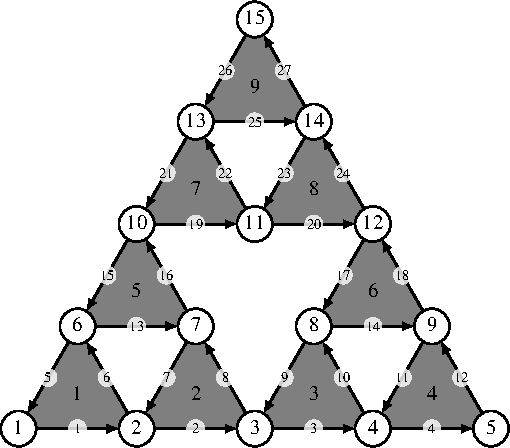
\includegraphics{chapters/95-homologie/images/gausshomoex.pdf}
\caption{Beispiel für die Berechnung von Basisvektoren und Homologieklassen
mit Hilfe des Gauss-Algorithmus
\label{buch:homologie:fig:gausshomoex}}
\end{figure}

\subsubsection{Basis von $Z_k(C)$}
Um eine Basis für $H_k(C)$ zu konstruieren, ist es zunächst nötig,
eine Basis der Zyklen $Z_k(C)$ zu bestimmen.
Ausgehend von einer beliebigen Basis der $C_k$ und einer 
zugehörigen Darstellung des Randoperators $\partial_k$ als
Matrix, kann eine Basis von Zyklen mit Hilfe des Gauss-Algorithmus
gefunden werden.
Wir bezeichnen die Menge dieser Zyklen mit
\[
\mathcal{Z}_k 
=
\{
z_1^{(k)},
z_2^{(k)},
\dots,
z_l^{(k)}
\}.
\]
$\mathcal{Z}_k$ erzeugt den $l$-dimensionalen Vektorraum $Z_k(C)$.

\begin{beispiel}
\label{buch:homologie:beispiel:gausshomo}
In Abbildung~\ref{buch:homologie:fig:gausshomoex} ist ein Polyeder 
dargestellt, dessen Homologiegruppe $H_1$ berechnet werden soll.
Um eine Basis für die Zyklen zu berechnen, wird zunächst die Matrix
des Randoperators $\partial_1$ aufgestellt.
Sie ist
\[
\setcounter{MaxMatrixCols}{27}
\partial_1
=
\footnotesize
\setlength\arraycolsep{2pt}
\begin{pmatrix*}[r]
%1  2  3  4  5  6  7  8  9 10 11 12 13 14 15 16 17 18 19 20 21 22 23 24 25 26 27
-1& 0& 0& 0&-1& 0& 0& 0& 0& 0& 0& 0& 0& 0& 0& 0& 0& 0& 0& 0& 0& 0& 0& 0& 0& 0& 0\\ % 1
 1&-1& 0& 0& 0&-1& 1& 0& 0& 0& 0& 0& 0& 0& 0& 0& 0& 0& 0& 0& 0& 0& 0& 0& 0& 0& 0\\ % 2
 0& 1&-1& 0& 0& 0& 0&-1& 1& 0& 0& 0& 0& 0& 0& 0& 0& 0& 0& 0& 0& 0& 0& 0& 0& 0& 0\\ % 3
 0& 0& 1&-1& 0& 0& 0& 0& 0&-1& 1& 0& 0& 0& 0& 0& 0& 0& 0& 0& 0& 0& 0& 0& 0& 0& 0\\ % 4
 0& 0& 0& 1& 0& 0& 0& 0& 0& 0& 0&-1& 0& 0& 0& 0& 0& 0& 0& 0& 0& 0& 0& 0& 0& 0& 0\\ % 5
 0& 0& 0& 0& 1& 1& 0& 0& 0& 0& 0& 0&-1& 0& 1& 0& 0& 0& 0& 0& 0& 0& 0& 0& 0& 0& 0\\ % 6
 0& 0& 0& 0& 0& 0&-1& 1& 0& 0& 0& 0& 1& 0& 0&-1& 0& 0& 0& 0& 0& 0& 0& 0& 0& 0& 0\\ % 7
 0& 0& 0& 0& 0& 0& 0& 0&-1& 1& 0& 0& 0&-1& 0& 0& 1& 0& 0& 0& 0& 0& 0& 0& 0& 0& 0\\ % 8
 0& 0& 0& 0& 0& 0& 0& 0& 0& 0&-1& 1& 0& 1& 0& 0& 0&-1& 0& 0& 0& 0& 0& 0& 0& 0& 0\\ % 9
 0& 0& 0& 0& 0& 0& 0& 0& 0& 0& 0& 0& 0& 0&-1& 1& 0& 0&-1& 0& 1& 0& 0& 0& 0& 0& 0\\ %10
 0& 0& 0& 0& 0& 0& 0& 0& 0& 0& 0& 0& 0& 0& 0& 0& 0& 0& 1&-1& 0&-1& 1& 0& 0& 0& 0\\ %11
 0& 0& 0& 0& 0& 0& 0& 0& 0& 0& 0& 0& 0& 0& 0& 0&-1& 1& 0& 1& 0& 0& 0&-1& 0& 0& 0\\ %12
 0& 0& 0& 0& 0& 0& 0& 0& 0& 0& 0& 0& 0& 0& 0& 0& 0& 0& 0& 0&-1& 1& 0& 0&-1& 1& 0\\ %13
 0& 0& 0& 0& 0& 0& 0& 0& 0& 0& 0& 0& 0& 0& 0& 0& 0& 0& 0& 0& 0& 0&-1& 1& 1& 0&-1\\ %14
 0& 0& 0& 0& 0& 0& 0& 0& 0& 0& 0& 0& 0& 0& 0& 0& 0& 0& 0& 0& 0& 0& 0& 0& 0&-1& 1\\ %15
\end{pmatrix*}
\]
Die reduzierte Zeilenstufenform von $\partial_1$ ist
(Pivotpositionen in {\color{red}rot}, frei wählbare Variablen
in {\color{darkgreen}grün})
\begin{center}
%\tiny
\scriptsize
%\footnotesize
\setlength\tabcolsep{3pt}
\begin{tabular}{|>{$}r<{$}|>{$}r<{$}>{$}r<{$}>{$}r<{$}>{$}r<{$}>{$}r<{$}>{$}r<{$}>{$}r<{$}>{$}r<{$}>{$}r<{$}>{$}r<{$}>{$}r<{$}>{$}r<{$}>{$}r<{$}>{$}r<{$}>{$}r<{$}>{$}r<{$}>{$}r<{$}>{$}r<{$}>{$}r<{$}>{$}r<{$}>{$}r<{$}>{$}r<{$}>{$}r<{$}>{$}r<{$}>{$}r<{$}>{$}r<{$}>{$}r<{$}|}
\hline
  & 1& 2& 3& 4& 5&{\color{darkgreen}6}& 7&{\color{darkgreen}8}& 9&{\color{darkgreen}10}&11&{\color{darkgreen}12}&{\color{darkgreen}13}&{\color{darkgreen}14}&15&{\color{darkgreen}16}&17&{\color{darkgreen}18}&19&{\color{darkgreen}20}&21&{\color{darkgreen}22}&23&{\color{darkgreen}24}&{\color{darkgreen}25}&26&{\color{darkgreen}27}\\
\hline
 1&\phantom{-}{\color{red}1}& 0& 0& 0& 0&-1& 0& 0& 0& 0& 0& 0& 1& 0& 0&-1& 0& 0& 0& 1& 0& 0& 0&-1& 0& 0& 0\\
 2& 0&\phantom{-}{\color{red}1}& 0& 0& 0& 0& 0&-1& 0& 0& 0& 0& 0& 0& 0& 0& 0& 0& 0& 1& 0& 0& 0&-1& 0& 0& 0\\
 3& 0& 0&\phantom{-}{\color{red}1}& 0& 0& 0& 0& 0& 0&-1& 0& 0& 0& 1& 0& 0& 0&-1& 0& 0& 0& 0& 0& 0& 0& 0& 0\\
 4& 0& 0& 0&\phantom{-}{\color{red}1}& 0& 0& 0& 0& 0& 0& 0&-1& 0& 0& 0& 0& 0& 0& 0& 0& 0& 0& 0& 0& 0& 0& 0\\
 5& 0& 0& 0& 0&\phantom{-}{\color{red}1}&-1& 0& 0& 0& 0& 0& 0& 1& 0& 0&-1& 0& 0& 0& 1& 0& 0& 0&-1& 0& 0& 0\\
 6& 0& 0& 0& 0& 0& 0&\phantom{-}{\color{red}1}&-1& 0& 0& 0& 0&-1& 0& 0& 1& 0& 0& 0& 0& 0& 0& 0& 0& 0& 0& 0\\
 7& 0& 0& 0& 0& 0& 0& 0& 0&\phantom{-}{\color{red}1}&-1& 0& 0& 0& 1& 0& 0& 0&-1& 0&-1& 0& 0& 0& 1& 0& 0& 0\\
 8& 0& 0& 0& 0& 0& 0& 0& 0& 0& 0&\phantom{-}{\color{red}1}&-1& 0&-1& 0& 0& 0& 1& 0& 0& 0& 0& 0& 0& 0& 0& 0\\
 9& 0& 0& 0& 0& 0& 0& 0& 0& 0& 0& 0& 0& 0& 0&\phantom{-}{\color{red}1}&-1& 0& 0& 0& 1& 0& 0& 0&-1& 0& 0& 0\\
10& 0& 0& 0& 0& 0& 0& 0& 0& 0& 0& 0& 0& 0& 0& 0& 0&\phantom{-}{\color{red}1}&-1& 0&-1& 0& 0& 0& 1& 0& 0& 0\\
11& 0& 0& 0& 0& 0& 0& 0& 0& 0& 0& 0& 0& 0& 0& 0& 0& 0& 0&\phantom{-}{\color{red}1}&-1& 0&-1& 0& 1& 1& 0&-1\\
12& 0& 0& 0& 0& 0& 0& 0& 0& 0& 0& 0& 0& 0& 0& 0& 0& 0& 0& 0& 0&\phantom{-}{\color{red}1}&-1& 0& 0& 1& 0&-1\\
13& 0& 0& 0& 0& 0& 0& 0& 0& 0& 0& 0& 0& 0& 0& 0& 0& 0& 0& 0& 0& 0& 0&\phantom{-}{\color{red}1}&-1&-1& 0& 1\\
14& 0& 0& 0& 0& 0& 0& 0& 0& 0& 0& 0& 0& 0& 0& 0& 0& 0& 0& 0& 0& 0& 0& 0& 0& 0&\phantom{-}{\color{red}1}&-1\\
15& 0& 0& 0& 0& 0& 0& 0& 0& 0& 0& 0& 0& 0& 0& 0& 0& 0& 0& 0& 0& 0& 0& 0& 0& 0& 0& 0\\
\hline
\end{tabular}.
\end{center}
Daraus kann man die Zyklen wie folgt ablesen, indem man jeweils
genau eine frei wählbare Variable auf $1$ setzt:
\begin{align*}
z_1
&=
\tiny
\begin{pmatrix*}[r]
\phantom{-}
 1\\
 0\\
 0\\
 0\\
 1\\
 1\\
 0\\
 0\\
 0\\
 0\\
 0\\
 0\\
 0\\
 0\\
 0\\
 0\\
 0\\
 0\\
 0\\
 0\\
 0\\
 0\\
 0\\
 0\\
 0\\
 0\\
 0
\end{pmatrix*},
&z_2
&=
\tiny
\begin{pmatrix*}[r]
\phantom{-}
 0\\
 1\\
 0\\
 0\\
 0\\
 0\\
 1\\
 1\\
 0\\
 0\\
 0\\
 0\\
 0\\
 0\\
 0\\
 0\\
 0\\
 0\\
 0\\
 0\\
 0\\
 0\\
 0\\
 0\\
 0\\
 0\\
 0
\end{pmatrix*},
&z_3
&=
\tiny
\begin{pmatrix*}[r]
\phantom{-}
 0\\
 0\\
 1\\
 0\\
 0\\
 0\\
 0\\
 0\\
 1\\
 1\\
 0\\
 0\\
 0\\
 0\\
 0\\
 0\\
 0\\
 0\\
 0\\
 0\\
 0\\
 0\\
 0\\
 0\\
 0\\
 0\\
 0
\end{pmatrix*},
&z_4 % variable 12 = 1
&=
\tiny
\begin{pmatrix*}[r]
\phantom{-}
 0\\
 0\\
 0\\
 1\\
 0\\
 0\\
 0\\
 0\\
 0\\
 0\\
 1\\
 1\\
 0\\
 0\\
 0\\
 0\\
 0\\
 0\\
 0\\
 0\\
 0\\
 0\\
 0\\
 0\\
 0\\
 0\\
 0
\end{pmatrix*},
&z_5 % variable 13 = 1
&=
\tiny
\begin{pmatrix*}[r]
-1\\
 0\\
 0\\
 0\\
-1\\
 0\\
 1\\
 0\\
 0\\
 0\\
 0\\
 0\\
 1\\
 0\\
 0\\
 0\\
 0\\
 0\\
 0\\
 0\\
 0\\
 0\\
 0\\
 0\\
 0\\
 0\\
 0
\end{pmatrix*},
&z_6 % variable 14 = 1
&=
\tiny
\begin{pmatrix*}[r]
 0\\
 0\\
-1\\
 0\\
 0\\
 0\\
 0\\
 0\\
-1\\
 0\\
 1\\
 0\\
 0\\
 1\\
 0\\
 0\\
 0\\
 0\\
 0\\
 0\\
 0\\
 0\\
 0\\
 0\\
 0\\
 0\\
 0
\end{pmatrix*},
&z_7 % variable 16 = 1
&=
\tiny
\begin{pmatrix*}[r]
 1\\
 0\\
 0\\
 0\\
 1\\
 0\\
-1\\
 0\\
 0\\
 0\\
 0\\
 0\\
 0\\
 0\\
 1\\
 1\\
 0\\
 0\\
 0\\
 0\\
 0\\
 0\\
 0\\
 0\\
 0\\
 0\\
 0
\end{pmatrix*},\\
z_8 % variable 18 = 1
&=
\tiny
\begin{pmatrix*}[r]
 0\\
 0\\
 1\\
 0\\
 0\\
 0\\
 0\\
 0\\
 1\\
 0\\
-1\\
 0\\
 0\\
 0\\
 0\\
 0\\
 1\\
 1\\
 0\\
 0\\
 0\\
 0\\
 0\\
 0\\
 0\\
 0\\
 0
\end{pmatrix*},
&z_9 % variable 20 = 1
&=
\tiny
\begin{pmatrix*}[r]
-1\\
-1\\
 0\\
 0\\
-1\\
 0\\
 0\\
 0\\
 1\\
 0\\
 0\\
 0\\
 0\\
 0\\
-1\\
 0\\
 1\\
 0\\
 1\\
 1\\
 0\\
 0\\
 0\\
 0\\
 0\\
 0\\
 0
\end{pmatrix*},
&z_{10} % variable 22 = 1
&=
\tiny
\begin{pmatrix*}[r]
\phantom{-}
 0\\
 0\\
 0\\
 0\\
 0\\ %5
 0\\ 
 0\\
 0\\
 0\\
 0\\ %10
 0\\ 
 0\\
 0\\
 0\\
 0\\ %15
 0\\
 0\\
 0\\
 1\\
 0\\ %20
 1\\
 1\\
 0\\
 0\\
 0\\ %25
 0\\
 0
\end{pmatrix*},
&z_{11} % variable 24 = 1
&=
\tiny
\begin{pmatrix*}[r]
 1\\
 1\\
 0\\
 0\\
 1\\ %5
 0\\
 0\\
 0\\
-1\\
 0\\ %10
 0\\
 0\\
 0\\
 0\\
 1\\ %15
 0\\
-1\\
 0\\
-1\\
 0\\ %20
 0\\
 0\\
 1\\
 1\\
 0\\ %25
 0\\
 0
\end{pmatrix*},
&z_{12} % variable 25 = 1
&=
\tiny
\begin{pmatrix*}[r]
 0\\
 0\\
 0\\
 0\\
 0\\
 0\\
 0\\
 0\\
 0\\
 0\\ %10
 0\\
 0\\
 0\\
 0\\
 0\\ %15
 0\\
 0\\
 0\\
-1\\
 0\\ %20
-1\\
 0\\
 1\\
 0\\
 1\\ %25
 0\\
 0
\end{pmatrix*},
&z_{13} % variable 27 = 1
&=
\tiny
\begin{pmatrix*}[r]
 0\\
 0\\
 0\\
 0\\
 0\\
 0\\
 0\\
 0\\
 0\\
 0\\
 0\\
 0\\
 0\\
 0\\
 0\\
 0\\
 0\\
 0\\
 1\\
 0\\ %20
 1\\
 0\\
-1\\
 0\\
 0\\ %25
 1\\
 1
\end{pmatrix*}
\end{align*}
\begin{figure}
\centering
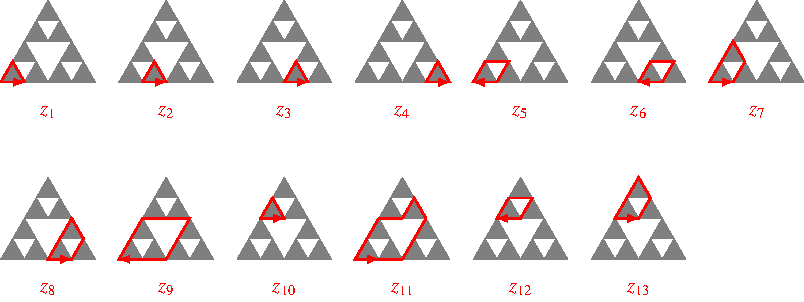
\includegraphics{chapters/95-homologie/images/homocycles.pdf}
\caption{Zyklen des Randoperators $\partial_1$ im Beispiel von
Seite~\pageref{buch:homologie:beispiel:gausshomo}.
\label{buch:homologie:fig:homocycles}}
\end{figure}%
Die Zyklen sind in Abbildung~\ref{buch:homologie:fig:homocycles} {\color{red}rot} dargestellt.
\end{beispiel}

\subsubsection{Basis für $B_k(C)$}
Da $B_k(C)\subset Z_k(C)$ gilt, lässt sich für jedes $c_{k+1}\in C_{k+1}$
der Rand $\partial_{k+1}c_{k+1}$ als Linearkombination der im 
vorangegangenen Schritt gefundenen Basiszyklen finden.
Wir können also aus der Standardbasis $e^{(k+1)}_i\in C_{k+1}$ eine Menge
von Vektoren $\partial_{k+1}e^{(k+1)}_i$ gewinnen, die mit Sicherheit
ganz $B_k(C)$ aufspannen.
Es ist aber davon auszugehen, dass diese Vektoren nicht linear unabhängig
sind.
Es ist also nötig, eine Teilmenge
\[
\mathcal{B}_k
=
\{
\partial_{k+1}e^{(k+1)}_{i_1},
\partial_{k+1}e^{(k+1)}_{i_2},
\dots,
\partial_{k+1}e^{(k+1)}_{i_m}
\}
\]
von Vektoren auszuwählen, die linear
unabhängig sind.
Diese bilden eine Basis von $B_k(C)$.

\begin{figure}
\centering
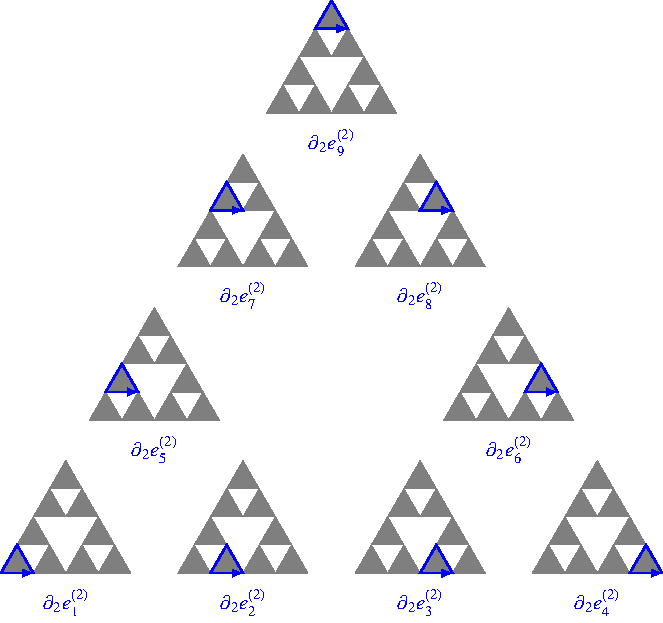
\includegraphics{chapters/95-homologie/images/homoboundaries.pdf}
\caption{Die Ränder $\partial_2e_i^{(2)}$ für das Beispiel von
Seite~\pageref{buch:homologie:beispiel:gausshomo}.
Die grauen Dreiecke bilden die Standardbasis $e_i^{(2)}$ von $C_2$,
die blauen Dreiecke sind die Ränder $\partial_2e_i^{(2)}$ dieser
Dreiecke.
\label{buch:homologie:fig:homoboundaries}}
\end{figure}

Aus den Abbildungen~\ref{buch:homologie:fig:homocycles} und
\ref{buch:homologie:fig:homoboundaries} kann man auch ablesen,
wie die Ränder $\partial_2e_i^{(2)}$ aus den Zyklen von $\mathcal{Z}_1$
linear kombiniert werden können.
Man erhält so die Beziehungen
\begin{equation}
\setcounter{MaxMatrixCols}{29}
\setlength\arraycolsep{1pt}
\begin{array}{lcrcrcrcrcrcrcrcrcrcrcrcrcr}
\partial_2e_1^{(2)} &=&z_1& &   & &   & &   & &   & &   & &   & &   & &   & &      & &      & &      & &      \\
\partial_2e_2^{(2)} &=&   & &z_2& &   & &   & &   & &   & &   & &   & &   & &      & &      & &      & &      \\
\partial_2e_3^{(2)} &=&   & &   & &z_3& &   & &   & &   & &   & &   & &   & &      & &      & &      & &      \\
\partial_2e_4^{(2)} &=&   & &   & &   & &z_4& &   & &   & &   & &   & &   & &      & &      & &      & &      \\
\partial_2e_5^{(2)} &=&   & &   & &   & &   & &z_5& &   &+&z_7& &   & &   & &      & &      & &      & &      \\
\partial_2e_6^{(2)} &=&   & &   & &   & &   & &   & &z_6& &   &+&z_8& &   & &      & &      & &      & &      \\
\partial_2e_7^{(2)} &=&   & &   & &   & &   & &   & &   & &   & &   & &   & &z_{10}& &      & &      & &      \\
\partial_2e_8^{(2)} &=&   & &   & &   & &   & &   & &   & &   & &   & &   & &      & &z_{11}& &      & &      \\
\partial_2e_9^{(2)} &=&   &\phantom{+}&   &\phantom{+} &   &\phantom{+} &   &\phantom{+} &   &\phantom{+} &   &\phantom{+} &   &\phantom{+} &   &\phantom{+} &   &\phantom{+} &      &\phantom{+} &      & &z_{12}&+&z_{13}
\end{array}
\end{equation}
Dies reicht jedoch nicht, um herauszufinden, welche der blauen Dreiecke
linear unabhängig sind.
Im vorliegenden Fall ist dies einfach: jedes blaue Dreieck besteht aus
Kanten, die in keinem anderen blauen Dreieck vorkommen, daher müssen
sie alle linear unabhängig sein.

\begin{figure}
\centering
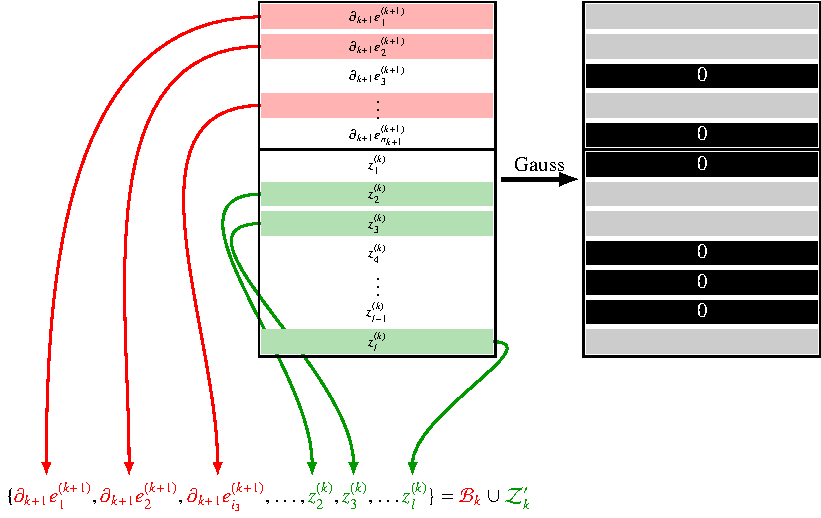
\includegraphics{chapters/95-homologie/images/gausshomobasis.pdf}
\caption{Bestimmung einer Basis für die Homologiegruppe $H_k(C)$ mit
Hilfe der Vorwärtsreduktion des Gaussalgorithmus.
Die schwarzen Nullzeilen zeigen an, welche Zeilenvektoren zusammen mit
den darüberliegenden Vektoren nicht linear unabhängig sind und damit nicht
in Frage kommen für die besuchte Basis.
Übrig bleiben die {\color{red}rot} und {\color{darkgreen}grün} hervorgehobenen
Vektoren.
\label{buch:homologie:fig:gausshomobasis}}
\end{figure}

Diese Auswahl lässt sich sehr leicht mit Hilfe der folgenden
Variante des Gauss-Algorithmus realisieren.
Dazu werden die $n_{k+1}$ Zeilen Gauss-Tableau zunächst mit den Vektoren
$\partial_{k+1}{e_i^{(k+1)}}^t$ gefüllt.
Führt man in diesem Tableau die Vorwärtsreduktion durch, wobei man
entstehende Nullzeilen einfach überspringt, bleiben nur noch Zeilen
übrig, die linear unabhängig sind.
Diese Zeilen entsprechen den linear unabhängigen Vektoren von $\mathcal{B}_k$,
die Zeilennummern sind $i_1,i_2,\dots,i_m$.
Dieses Vorgehen ist schematisch im oberen Teil der
Abbildung~\ref{buch:homologie:fig:gausshomobasis} dargestellt.

\subsubsection{Basis für die Homologiegruppe $H_k(C)$}
Um eine Basis von $H_k(C)$ zu konstruieren, müssen wir jetzt eine
Basis von Zyklen finden, die sich nicht nur um einen Rand unterscheiden,
die also zu verschiedenen Homologie-Klassen in $H_k(C)$ gehören.
Gesucht sind jetzt also Vektoren $\mathcal{Z}'_k$ derart, dass 
die Vektoren von $\mathcal{Z}'_k\cup\mathcal{B}_k$ immer noch $Z_k(C)$
aufspannen, aber zusätzlich linear unabhängig sind.

Dazu kann man wie folgt vorgehen.
\begin{enumerate}
\item
Man beginnt mit $\mathcal{D}_0=\emptyset$ und setzt $j=0$.
\item
Dann testet man der Reihe nach alle noch nicht getesteten Vektoren
von $z_i^{(k)}\in\mathcal{Z}_k$ daraufhin, ob sie von den Vektoren
$\mathcal{B}_k\cup \mathcal{D}_j$ linear unabhängig sind.
Wenn ja, bildet man $\mathcal{D}_{j+1} = \mathcal{D}\cup\{z^{(k)}_i\}$ und
setzt $j=1$.
Andernfalls ignoriert man $z^{(k)}_i$.
\item
Schritt 2 wird wiederholt, bis man alle Vektoren von $\mathcal{Z}_k$
getestet hat.
Die gesuchte Basis setzt sich zusammen  aus $\mathcal{B}_k$ und
$\mathcal{D}_l$,
also
$
\mathcal{Z}_k'
=
\mathcal{B}_k
\cup
\mathcal{D}_l.
$
\end{enumerate}

Dieser Algorithmus kann ebenfalls mit der oben angesprochenen Variante
des Gauss-Algorithmus durchgeführt werden.
Dazu werden die Zeilen $n_k+1$ bis $n_k+1+|\mathcal{Z}_k|$ mit den
Vektoren $z_i^t$.
Dann führt man die Vorwärtsreduktion im ganzen Tableau durch, wobei
man wieder die Nullzeilen stehen lässt.
Nullzeilen zeigen wieder Vektoren an, die sich linear durch die darüber
liegenden Vektoren ausdrücken lassen.
Die auszuwählenden Vektoren sind daher genau diejenigen, die für
$\mathcal{Z}_k'$ ausgewählt werden müssen.

Um den Algorithmus durchzuführen, bilden wir daher das Gauss-Tableau
in Abbildung~\ref{buch:homologie:beispiel:gausstableau},
bestehend aus den Vektoren $\partial_2e_i^{(2)}$ in den ersten 9
Zeilen und den Zyklen $z_1,\dots,z_{13}$ in den folgenden 13 Zeilen.
Das reduzierte Tableau nach der Vorwärtsreduktion ist in
Abbildung~\ref{buch:homologie:beispiel:gausstableaureduziert}
dargestellt, amn erkennt, dass die Zyklen $z_1$ bis $z_4$, $z_7$ und $z_8$,
$z_9$ und $z_{10}$ sowie $z_{13}$ weggelassen werden müssen.
Es bleiben die folgenden Zyklen:
\begin{center}
\begin{tabular}{>{$}l<{$}l}
\text{Zyklus}&Eigenschaft\\
\hline
z_5   &Zyklus umschliesst das kleine weisse Dreieck links unten\\
z_6   &Zyklus umschliesst das kleine weisse Dreieck rechts unten\\
z_9   &Zyklus umschliesst das grosse weisse Dreieck\\
z_{12}&Zyklus umschliesst das kleine weisse Dreicke oben\\
\hline
\end{tabular}
\end{center}
Die Zyklen, die nach der Reduktion übrig bleiben, sind in
Abbildung~\ref{buch:homologie:beispiel:homoclasses} zusammengestellt.
Jede solche Klasse entspricht genau einem der ``Löcher'', der weissen
Dreiecke.
Die Homologie kann man also als eine exakte Version der Idee eines
Vektorraums erzeugt von den ``Löchern'' eines Polygons verstehen.

\begin{figure}
\centering
\setlength\tabcolsep{1pt}
\begin{tabular}{|>{$}c<{$}|>{$}r<{$}>{$}r<{$}>{$}r<{$}>{$}r<{$}>{$}r<{$}>{$}r<{$}>{$}r<{$}>{$}r<{$}>{$}r<{$}>{$}r<{$}|>{$}r<{$}>{$}r<{$}>{$}r<{$}>{$}r<{$}>{$}r<{$}>{$}r<{$}>{$}r<{$}>{$}r<{$}>{$}r<{$}>{$}r<{$}|>{$}r<{$}>{$}r<{$}>{$}r<{$}>{$}r<{$}>{$}r<{$}>{$}r<{$}>{$}r<{$}|}
\hline
&\scriptstyle 1&\scriptstyle 2&\scriptstyle 3&\scriptstyle 4 &\scriptstyle 5
&\scriptstyle 6 &\scriptstyle 7 &\scriptstyle 8 &\scriptstyle 9 &\scriptstyle 10
&\scriptstyle 11 &\scriptstyle 12 &\scriptstyle 13 &\scriptstyle 14 &\scriptstyle 15
&\scriptstyle 16 &\scriptstyle 17 &\scriptstyle 18 &\scriptstyle 19 &\scriptstyle 20
&\scriptstyle 21 &\scriptstyle 22 &\scriptstyle 23 &\scriptstyle 24 &\scriptstyle 25
&\scriptstyle 26 &\scriptstyle 27
\\
%                                1  2  3  4  5  6  7  8  9  0  1  2  3  4  5  6  7  8  9  0  1  2  3  4  5  6  7
\hline
\scriptstyle\partial_2e_1^{(2)}& 1&  &  &  & 1&\phantom{-}1&  &  &  &  &  &  &  &  &  &  &  &  &  &  &  &  &  &  &  &  &  \\
\scriptstyle\partial_2e_2^{(2)}&  & 1&  &  &  &  & 1&\phantom{-}1&  &  &  &  &  &  &  &  &  &  &  &  &  &  &  &  &  &  &  \\
\scriptstyle\partial_2e_3^{(2)}&  &  & 1&  &  &  &  &  &\phantom{-}1&\phantom{-}1&  &  &  &  &  &  &  &  &  &  &  &  &  &  &  &  &  \\
\scriptstyle\partial_2e_4^{(2)}&  &  &  &\phantom{-}1&  &  &  &  &  &  & 1&\phantom{-}1&  &  &  &  &  &  &  &  &  &  &  &  &  &  &  \\
\scriptstyle\partial_2e_5^{(2)}&  &  &  &  &  &  &  &  &  &  &  &  & 1&  & 1&\phantom{-}1&  &  &  &  &  &  &  &  &  &  &  \\
\scriptstyle\partial_2e_6^{(2)}&  &  &  &  &  &  &  &  &  &  &  &  &  &\phantom{-}1&  &  & 1&\phantom{-}1&  &  &  &  &  &  &  &  &  \\
\scriptstyle\partial_2e_7^{(2)}&  &  &  &  &  &  &  &  &  &  &  &  &  &  &  &  &  &  & 1&  &\phantom{-}1& 1&  &  &  &  &  \\
\scriptstyle\partial_2e_8^{(2)}&  &  &  &  &  &  &  &  &  &  &  &  &  &  &  &  &  &  &  &\phantom{-}1&  &  & 1&\phantom{-}1&  &  &  \\
\scriptstyle\partial_2e_9^{(2)}&  &  &  &  &  &  &  &  &  &  &  &  &  &  &  &  &  &  &  &  &  &  &  &  &\phantom{-}1&\phantom{-}1&\phantom{-}1\\
\hline
%                    1  2  3  4  5  6  7  8  9 10 11 12 13 14 15 16 17 18 19 20 21 22 23 24 25 26 27
\scriptstyle z_{ 1}& 1&  &  &  & 1& 1&  &  &  &  &  &  &  &  &  &  &  &  &  &  &  &  &  &  &  &  &  \\
\scriptstyle z_{ 2}&  & 1&  &  &  &  & 1& 1&  &  &  &  &  &  &  &  &  &  &  &  &  &  &  &  &  &  &  \\
\scriptstyle z_{ 3}&  &  & 1&  &  &  &  &  & 1& 1&  &  &  &  &  &  &  &  &  &  &  &  &  &  &  &  &  \\
\scriptstyle z_{ 4}&  &  &  & 1&  &  &  &  &  &  & 1& 1&  &  &  &  &  &  &  &  &  &  &  &  &  &  &  \\
\scriptstyle z_{ 5}&-1&  &  &  &-1&  & 1&  &  &  &  &  & 1&  &  &  &  &  &  &  &  &  &  &  &  &  &  \\
\scriptstyle z_{ 6}&  &  &-1&  &  &  &  &  &-1&  & 1&  &  & 1&  &  &  &  &  &  &  &  &  &  &  &  &  \\
\scriptstyle z_{ 7}& 1&  &  &  & 1&  &-1&  &  &  &  &  &  &  & 1& 1&  &  &  &  &  &  &  &  &  &  &  \\
\scriptstyle z_{ 8}&  &  & 1&  &  &  &  &  & 1&  &-1&  &  &  &  &  & 1& 1&  &  &  &  &  &  &  &  &  \\
\scriptstyle z_{ 9}&-1&-1&  &  & 1&  &  &  & 1&  &  &  &  &  &-1&  & 1& 1& 1&  &  &  &  &  &  &  &  \\
\scriptstyle z_{10}&  &  &  &  &  &  &  &  &  &  &  &  &  &  &  &  &  & 1&  & 1& 1&  &  &  &  &  &  \\
\scriptstyle z_{11}& 1& 1&  &  & 1&  &  &  &-1&  &  &  &  &  & 1&  &-1&  &-1&  &  &  & 1& 1&  &  &  \\
\scriptstyle z_{12}&  &  &  &  &  &  &  &  &  &  &  &  &  &  &  &  &  &  &-1&  &-1&  & 1&  & 1&  &  \\
\scriptstyle z_{13}&  &  &  &  &  &  &  &  &  &  &  &  &  &  &  &  &  &  & 1&  & 1&  &-1&  &  & 1& 1\\
\hline
\end{tabular}
\caption{Gauss-Tableau für die Bestimmung einer Basis von
$H_1$ für das Beispiel. 
Die ersten neuen Zeilen bestehen aus den Bildern der
Basisvektoren von $C_2$.
Im vorliegenden Fall kann man sofort sehen, dass alle diese
Zeilen linear unabhängig sind.
Die folgenden Zeilen sind die Zyklen in $\mathbb{Z}_2$, sie
sind ebenfalls linear unabhängig.
Mit Hilfe der Vorwärtsreduktion müssen jetzt diejenigen
Zeilen elminiert werden, die bereits aus anderen Zyklen
mit Hilfe von Rändern der Zeilen 1--9 kombiniert werden können.
\label{buch:homologie:beispiel:gausstableau}}
\end{figure}

\begin{figure}
\centering
\setlength\tabcolsep{1pt}
\begin{tabular}{|>{$}c<{$}|>{$}r<{$}>{$}r<{$}>{$}r<{$}>{$}r<{$}>{$}r<{$}>{$}r<{$}>{$}r<{$}>{$}r<{$}>{$}r<{$}>{$}r<{$}|>{$}r<{$}>{$}r<{$}>{$}r<{$}>{$}r<{$}>{$}r<{$}>{$}r<{$}>{$}r<{$}>{$}r<{$}>{$}r<{$}>{$}r<{$}|>{$}r<{$}>{$}r<{$}>{$}r<{$}>{$}r<{$}>{$}r<{$}>{$}r<{$}>{$}r<{$}|}
\hline
&\scriptstyle 1&\scriptstyle 2&\scriptstyle 3&\scriptstyle 4 &\scriptstyle 5
&\scriptstyle 6 &\scriptstyle 7 &\scriptstyle 8 &\scriptstyle 9 &\scriptstyle 10
&\scriptstyle 11 &\scriptstyle 12 &\scriptstyle 13 &\scriptstyle 14 &\scriptstyle 15
&\scriptstyle 16 &\scriptstyle 17 &\scriptstyle 18 &\scriptstyle 19 &\scriptstyle 20
&\scriptstyle 21 &\scriptstyle 22 &\scriptstyle 23 &\scriptstyle 24 &\scriptstyle 25
&\scriptstyle 26 &\scriptstyle 27
\\
%                                1  2  3  4  5  6  7  8  9  0  1  2  3  4  5  6  7  8  9  0  1  2  3  4  5  6  7
\hline
\scriptstyle\partial_2e_1^{(2)}&\phantom{-}1&  &  &  &\phantom{-}1&\phantom{-}1&  &  &  &  &  &  &  &  &  &  &  &  &  &  &  &  &  &  &  &  &  \\
\scriptstyle\partial_2e_2^{(2)}&  &\phantom{-}1&  &  &  &  &\phantom{-}1&\phantom{-}1&  &  &  &  &  &  &  &  &  &  &  &  &  &  &  &  &  &  &  \\
\scriptstyle\partial_2e_3^{(2)}&  &  &\phantom{-}1&  &  &  &  &  &\phantom{-}1&\phantom{-}1&  &  &  &  &  &  &  &  &  &  &  &  &  &  &  &  &  \\
\scriptstyle\partial_2e_4^{(2)}&  &  &  &\phantom{-}1&  &  &  &  &  &  &\phantom{-}1&\phantom{-}1&  &  &  &  &  &  &  &  &  &  &  &  &  &  &  \\
\scriptstyle\partial_2e_5^{(2)}&  &  &  &  &  &  &  &  &  &  &  &  & 1&  & 1&\phantom{-}1&  &  &  &  &  &  &  &  &  &  &  \\
\scriptstyle\partial_2e_6^{(2)}&  &  &  &  &  &  &  &  &  &  &  &  &  &\phantom{-}1&  &  & 1&\phantom{-}1&  &  &  &  &  &  &  &  &  \\
\scriptstyle\partial_2e_7^{(2)}&  &  &  &  &  &  &  &  &  &  &  &  &  &  &  &  &  &  & 1&  &\phantom{-}1& 1&  &  &  &  &  \\
\scriptstyle\partial_2e_8^{(2)}&  &  &  &  &  &  &  &  &  &  &  &  &  &  &  &  &  &  &  &\phantom{-}1&  &  & 1&\phantom{-}1&  &  &  \\
\scriptstyle\partial_2e_9^{(2)}&  &  &  &  &  &  &  &  &  &  &  &  &  &  &  &  &  &  &  &  &  &  &  &  &\phantom{-}1&\phantom{-}1&\phantom{-}1\\
\hline
%                     1  2  3  4  5  6  7  8  9 10 11 12 13 14 15 16 17 18 19 20 21 22 23 24 25 26 27
\scriptstyle z_{ 1}'&  &  &  &  &  &  &  &  &  &  &  &  &  &  &  &  &  &  &  &  &  &  &  &  &  &  &  \\
\scriptstyle z_{ 2}'&  &  &  &  &  &  &  &  &  &  &  &  &  &  &  &  &  &  &  &  &  &  &  &  &  &  &  \\
\scriptstyle z_{ 3}'&  &  &  &  &  &  &  &  &  &  &  &  &  &  &  &  &  &  &  &  &  &  &  &  &  &  &  \\
\scriptstyle z_{ 4}'&  &  &  &  &  &  &  &  &  &  &  &  &  &  &  &  &  &  &  &  &  &  &  &  &  &  &  \\
\scriptstyle z_{ 5}'&  &  &  &  &  & 1& 1&  &  &  &  &  &  &  &-1&-1&  &  &  &  &  &  &  &  &  &  &  \\
\scriptstyle z_{ 6}'&  &  &  &  &  &  &  &  &  & 1& 1&  &  &  &  &  &-1&-1&  &  &  &  &  &  &  &  &  \\
\scriptstyle z_{ 7}'&  &  &  &  &  &  &  &  &  &  &  &  &  &  &  &  &  &  &  &  &  &  &  &  &  &  &  \\
\scriptstyle z_{ 8}'&  &  &  &  &  &  &  &  &  &  &  &  &  &  &  &  &  &  &  &  &  &  &  &  &  &  &  \\
\scriptstyle z_{ 9}'&  &  &  &  &  &  &  & 1& 1&  &  &  &  &  &  & 1& 1&  &  &  &-1&-1&-1&-1&  &  &  \\
\scriptstyle z_{10}'&  &  &  &  &  &  &  &  &  &  &  &  &  &  &  &  &  &  &  &  &  &  &  &  &  &  &  \\
\scriptstyle z_{11}'&  &  &  &  &  &  &  &  &  &  &  &  &  &  &  &  &  &  &  &  &  &  &  &  &  &  &  \\
\scriptstyle z_{12}'&  &  &  &  &  &  &  &  &  &  &  &  &  &  &  &  &  &  &  &  &  & 1& 1&  &  &-1&-1\\
\scriptstyle z_{13}'&  &  &  &  &  &  &  &  &  &  &  &  &  &  &  &  &  &  &  &  &  &  &  &  &  &  &  \\
\hline
\end{tabular}
\caption{Nach Durchführung der Vorwärtsreduktion kann man die Zyklen
ablesen, die nicht für eine Basis von $H_1$ gebraucht werden.
Die resultierenden Zyklen sind in Abbildung~\ref{buch:homologie:beispiel:homoclasses}
dargestellt.
\label{buch:homologie:beispiel:gausstableaureduziert}}
\end{figure}

\begin{figure}
\centering
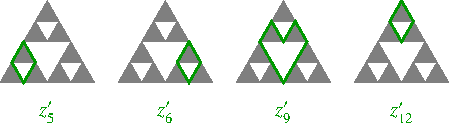
\includegraphics{chapters/95-homologie/images/homoclasses.pdf}
\caption{Repräsentanten für die reduzierten Klassen aus dem
Tableau von
Abbildung~\ref{buch:homologie:beispiel:gausstableaureduziert},
sie bilden eine Basis der Homologie-Gruppe $H_1$.
Jeder dieser Repräsentanten umschliesst genau ein ``Loch'',
also genau ein weisses Dreieck.
\label{buch:homologie:beispiel:homoclasses}}
\end{figure}

\subsubsection{Basis von $H_k(C)$}
Die im vorangegangenen Abschnitt konstruierte Basis kann jetzt auch
dazu verwendet werden, eine Basis von $H_k(C)$ zu finden.
Die Vektoren in $\mathcal{B}_k$ bilden eine Basis von $B_k(C)$
und die Vektoren in $\mathcal{Z}_k'$ sind davon unabhängig.
Die Klassen der Vektoren von $\mathcal{Z}_k'$ in $H_k(C)$ sind
daher ebenfalls linear unabhängig und bilden damit eine Basis
von $H_k(C)$.
Die von obigem Algorithmus ausgewählten Zyklen bilden also automatisch
eine Basis von Zyklen, die nicht Rand irgend einer Kette in $C_{k+1}$
sein können.

\subsection{Euler-Charakteristik}
Die Homologiegruppen fassen die Idee, die ``Löcher'' in 
Dimension $k$ eines Polyeders zu zählen, algebraisch exakt.
Dazu ist aber die algebraische Struktur von $H_k(C)$  gar 
nicht nötig, nur schon die Dimension des Vektorraumes $H_k(C)$
liefert bereits die verlange Information.

Dies ist auch der Ansatz, den der eulersche Polyedersatz verfolgt.
Euler hat für dreidimensionale Polyeder eine Invariante gefunden, 
die unabhängig ist von der Triangulation.

\begin{definition}
\label{buch:homologie:def:eulerchar}
Ist $E$ die Anzahl der Ecken, $K$ die Anzahl der Kanten und $F$
die Anzahl der Flächen eines dreidimensionalen Polyeders $P$, dann
heisst
\[
\chi(P) = E-K+F
\]
die {\em Euler-Charakteristik} des Polyeders $P$.
\end{definition}

Der Eulersche Polyedersatz, den wir nicht gesondert beweisen
wollen, besagt, dass $\chi(P)$ unabhängig ist von der 
Triangulation.
Alle regelmässigen Polyeder sind verschiedene Triangulationen
einer Kugel, sie haben alle den gleichen Wert $2$
der Euler-Charakteristik.

Ändert man die Triangulation, dann wird die Dimension der
Vektorräume $B_k(C)$ und $Z_k(C)$ grösser werden.
Kann man eine Grösse analog zu $\chi(P)$ finden, die sich nicht ändert?

\begin{definition}
Sei $C$ ein Kettenkomplex, dann heisst
\[
\chi(C) = \sum_{k=0}^n (-1)^k\dim H_k(C)
\]
die Euler-Charakteristik von $C$.
\end{definition}

Die Definition verlangt, dass man erst die Homologiegruppen
berechnen muss, bevor man die Euler-Charakteristik bestimmen
kann.
Dies ist aber in vielen Fällen gar nicht nötig, da dies nur
eine Frage der Dimensionen ist, die man direkt aus den
$C_k$ ablesen kann, wie wir nun zeigen wollen.

Die Dimension der Homologiegruppen ist
\begin{equation}
\dim H_k(C)
=
\dim \bigl(Z_k(C) / B_k(C)\bigr)
=
\dim Z_k(C) - \dim B_k(C).
\label{buch:homologie:eqn:dimHk}
\end{equation}
Die Bestimmung der Dimensionen der Zyklen und Ränder erfordert
aber immer noch, dass wir dafür Basen bestimmen müssen, es ist
also noch nichts eingespart.
Die Zyklen bilden den Kern von $\partial$, also 
\[
\dim Z_k(C) = \dim\ker \partial_k.
\]
Die Ränder $B_k(C)$ sind die Bilder von $\partial_{k+1}$, also
\[
\dim B_k(C)
=
\dim C_{k+1} - \ker\partial_{k+1}
=
\dim C_{k+1} - \dim Z_{k+1}(C).
\]
Daraus kann man jetzt eine Formel für die Euler-Charakteristik
gewinnen.
Sie ist
\begin{align*}
\chi(C)
&=
\sum_{k=0}^\infty (-1)^k \dim H_k(C)
\\
&=
\sum_{k=0}^\infty (-1)^k \bigl(\dim Z_k(C) - \dim B_k(C)\bigr)
\\
&=
\sum_{k=0}^\infty (-1)^k \dim Z_k(C) 
-
\sum_{k=0}^\infty (-1)^k \bigl(\dim C_{k+1} - \dim_{k+1}(C)\bigr)
\\
&=
-\sum_{k=0}^\infty (-1)^k \dim C_{k+1} 
+
\sum_{k=0}^\infty (-1)^k \dim Z_k(C) 
+
\sum_{k=0}^\infty (-1)^k \dim Z_{k+1}(C).
\intertext{Indem wir in der letzten Summe den Summationsindex $k$ durch
$k-1$ ersetzen, können wir bis auf den ersten Term die Summen
der $\dim Z_k(C)$ zum Verschwinden bringen:}
&=
-\sum_{k=0}^\infty (-1)^k \dim C_{k+1} 
+
\sum_{k=0}^\infty (-1)^k \dim Z_k(C) 
-
\sum_{k=1}^\infty (-1)^k \dim Z_k(C)
\\
&=
\sum_{k=1}^\infty (-1)^k \dim C_{k}
+
\dim \underbrace{Z_0(C)}_{\displaystyle =C_0}.
\intertext{In der letzten Umformung haben wir auch in der ersten
Summe den Summationsindex $k$ durch $k-1$ ersetzt.
Damit beginnt die Summation bei $k=1$.
Der fehlende Term ist genau der Term, der von den Summen der
$\dim Z_k(C)$ übrig bleibt.
Damit erhalten wir}
&=
\sum_{k=0}^\infty (-1)^k \dim C_{k}.
\end{align*}

\begin{satz}
Für die Euler-Charakteristik eines endlichdimensionalen Kettenkomplexes $C$ gilt
\[
\chi(C)
=
\sum_{k=0}^\infty (-1)^k \dim H_k(C)
=
\sum_{k=0}^\infty (-1)^k \dim C_k.
\]
\end{satz}
Im nächsten Abschnitt wird gezeigt, dass die Euler-Charakteristik
als Spezialfall der Lefshetz-Zahl verstanden werden kann.

\subsection{Induzierte Abbildung
\label{buch:subsection:induzierte-abbildung}}
Früher haben wurde eine Abbildung $f_*$ zwischen Kettenkomplexen $C_*$ und
$D_*$ so definiert,
dass sie mit den Randoperatoren verträglich sein muss.
Diese Forderung bewirkt, dass sich auch eine lineare Abbildung
\[
H_k(f) \colon H_k(C) \to H_k(D)
\]
zwischen den Homologiegruppen ergibt, wie wir nun zeigen wollen.

\subsubsection{Definition der induzierten Abbildung}
Um eine Abbildung von $H_k(C)$ nach $H_k(D)$ zu definieren, müssen wir
zu einem Element von $H_k(C)$ ein Bildelement konstruieren.
Ein Element in $H_k(C)$ ist eine Menge von Zyklen in $Z^C_k$, die sich
nur um einen Rand in $B_k$ unterscheiden.
Wir wählen also einen Zyklus $z\in Z_k$ und bilden ihn auf $f_k(z)$ ab.
Wegen $\partial^D_kf(z)=f\partial^C_kz = f(0) =0 $ ist auch $f_k(z)$
ein Zyklus.
Wir müssen jetzt aber noch zeigen, dass eine andere Wahl des Zyklus
das gleiche Element in $H_k(D)$ ergibt.
Dazu genügt es zu sehen, dass sich $f(z)$ höchstens um einen Rand
ändert, wenn man $z$ um einen Rand ändert.
Sei also $b\in B^C_k$ ein Rand, es gibt also ein $w\in C_{k+1}$ mit
$\partial^C_{k+1}w=b$.
Dann gilt aber auch
\[
f_k(z+b)
=
f_k(z) + f_k(b)
=
f_k(z) + f_k(\partial^C_{k+1}w)
=
f_k(z) + \partial^D_{k+1}(f_k(w)).
\]
Der letzte Term ist ein Rand in $D_k$, somit ändert sich $f_k(z)$ nur
um diesen Rand, wenn man $z$ um einen Rand ändert.
$f_k(z)$ und $f_k(z+b)$ führen auf die selbe Homologieklasse.

\subsubsection{Matrixdarstellung}
In Abschnitt~\ref{buch:subsection:basiswahl} wurde gezeigt, wie man
für die Vektorräume der Zyklen eine Basis derart finden kann, 
dass die Ränder von einer Teilmenge der Basis aufgespannt werden.
Eine solche Basis kann man immer erweitern zu einer Basis von $C_k$.
Für das Folgende bezeichnen wir die Vektoren einer solche Basis von $C_k$ 
mit
\[
\{
b_1,\dots, b_r,
z_1,\dots,z_l,
c_1,\dots,c_s
\}.
\]
wobei die Vektoren  die folgende Bedeutung haben:
\begin{center}
\begin{tabular}{|l|l|}
\hline
Vektoren&Bedeutung\\
\hline
$b_1,\dots,b_r$ & Basis für $B_k(C)$ \\
$z_1,\dots,z_l$ & zusätzliche Vektoren für eine Basis von $Z_k(C)$ \\
$c_1,\dots,c_s$ & zusätzliche Vektoren für eine Basis von $C_k$ \\
\hline
\end{tabular}
\end{center}

Wählt man eine Basis dieser Art sowohl in $C_*$ wie auch in $D_*$,
dann kann man die induzierte Abbildung als $3\times 3$-Blockmatrix
schreiben.
Man verwendet dabei, dass $f_k$ die Unterräume $B_k(C)$ und
$Z_k(C)$ in die entsprechenden Unterräume $B_k(D)$ und $Z_k(D)$
abbildet, also
\[
f_k(B_k(C)) \subset B_k(D)
\qquad\text{und}\qquad
f_k(Z_k(C)) \subset Z_k(D).
\]
In der Matrixdarstellung äussert sich das darin, dass die Blöcke
links unten zu Null werden.
Die Matrixdarstellung von $f_k$ hat daher die Form
\[
f_k
=
\begin{pmatrix}
f_{k,B} &    *    & * \\
   0    & f_{k,Z} & * \\
   0    &    0    & f_{k,*}
\end{pmatrix}.
\]
Genauso kann man natürlich auch die Randoperatoren in dieser Basis
ausdrücken.
Sie bilden die Zyklen auf $0$ ab und aus den Vektoren $c_1,\dots,c_s$
werden Ränder.
Die Matrix hat daher die Form
\[
\partial_k
=
\begin{pmatrix}
0& 0 & \Delta_k \\
0& 0 & 0 \\
0& 0 & 0
\end{pmatrix}
\]
\begin{figure}
\centering
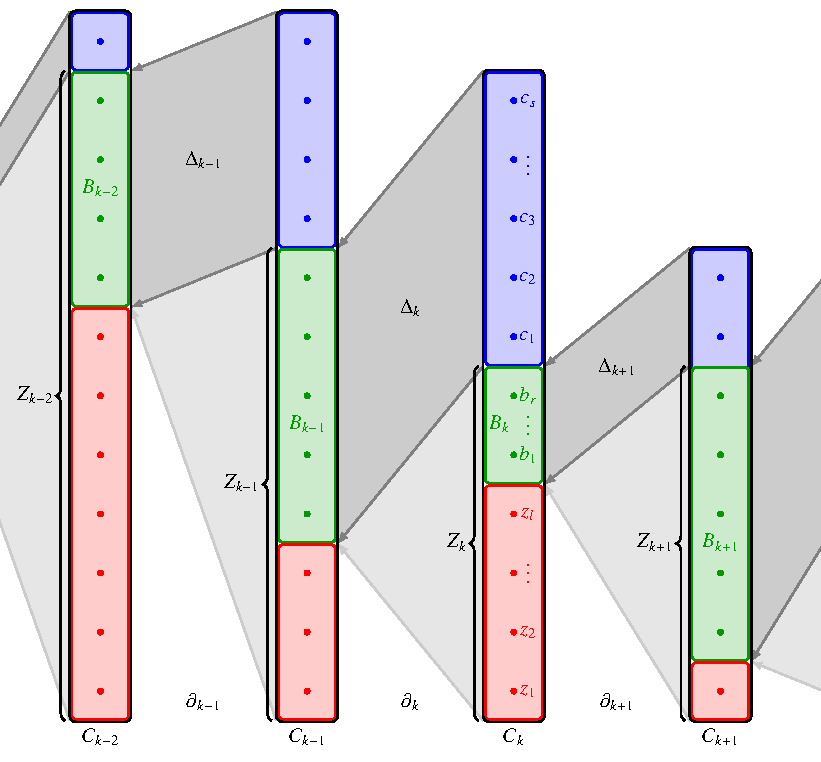
\includegraphics{chapters/95-homologie/images/complexbasis.pdf}
\caption{Basiswahl für den Kettenkomplex $C_k$.
Der Randoperator $\partial_k$ bildet $Z_k$ auf $0$ ab, der blaue
Unterraum, aufgespannt von den Vektoren $c_i$, wird bijektiv auf $B_{k-1}$
abgebildet.
Eine Basis kann immer so gefunden werden, dass die Vektoren $c_i$ 
von $\partial_k$ auf die Basisvektoren von $B_{k-1}$ abgebildet werden.
In dieser Basis ist $\Delta_k$ eine Einheitsmatrix.
\label{buch:homologie:fig:komplexbasis}}
\end{figure}%
Die Bedingung \eqref{buch:komplex:abbildung} für die Komplexabbildung
bekommt jetzt die Matrixform
\begin{equation}
\left.
\begin{aligned}
\partial_k^{D}\circ f_k
&=
\begin{pmatrix}
0&0&\Delta_k^{(D)}\\
0&0&0\\
0&0&0
\end{pmatrix}
\begin{pmatrix}
f_{k,B} &    *    & * \\
   0    & f_{k,Z} & * \\
   0    &    0    & f_{k,*}
\end{pmatrix}
=
\begin{pmatrix}
0&0&\Delta_k^{(D)}f_{k,*}\\
0&0&0\\
0&0&0
\end{pmatrix}
\\
f_{k-1}\circ \partial_k^C
&=
\begin{pmatrix}
f_{k-1,B}&   *   &   *   \\
   0   &f_{k-1,Z}&   *   \\
   0   &   0   &f_{k-1,*}
\end{pmatrix}
\begin{pmatrix}
0&0&\Delta_k^{(C)}\\
0&0&0\\
0&0&0
\end{pmatrix}
=
\begin{pmatrix}
0&0&f_{k-1,B}\Delta_k^{(C)}\\
0&0&0\\
0&0&0
\end{pmatrix}
\end{aligned}
\right\}
\Rightarrow
\Delta_k^{(D)}f_{k,*}
=
f_{k-1,B}\Delta_k^{(C)}.
\label{buch:homologie:matrixform}
\end{equation}
Für die induzierte Abbildung in Homologie ist ausschliesslich der
Block $f_{k,Z}$ notwendig, die Matrix von $H_k(f)$ in der gewählten
Basis von $H_k(C)$ bzw.~$H_k(D)$ ist also genau die Matrix $f_{k,Z}$.


Wie Abbildung~\ref{buch:homologie:fig:komplexbasis} können die
Basisvektoren $c_*$ in $C_k$ so gewählt werden, dass sie vom Randoperator
$\partial_k$ auf die Basisvektoren von $Z_{k-1}$ abgebildet werden.
Bei dieser Wahl wird die Matrix $\Delta_k$ eine Einheitsmatrix.

\subsubsection{Spur}
Wir betrachten jetzt den Fall einer Selbstabbildung $f_*\colon C_*\to C_*$.
Die Basis soll so gewählt werden, dass $\Delta_k$ eine Einheitsmatrix ist.
Aus~\eqref{buch:homologie:matrixform} kann man ablesen, dass für diese
Basiswahl $f_{k,*}=f_{k-1,B}$ gilt.
Die Matrizen von $f_k$ haben daher die Form
\[
f_k
=
\begin{pmatrix}
f_{k,B} &    *    & * \\
   0    & f_{k,Z} & * \\
   0    &   0     & f_{k-1,B}
\end{pmatrix}.
\]
Entsprechend ist die Spur
\begin{equation}
\operatorname{Spur} f_k
=
\operatorname{Spur} f_{k,B}
+
\operatorname{Spur} f_{k,Z}
+
\operatorname{Spur} f_{k-1,B}.
\label{buch:homologie:eqn:spur}
\end{equation}





